\documentclass[11pt]{article}
\usepackage{graphicx}
\usepackage{hyperref}
\usepackage{natbib}
\usepackage{amsmath}
\usepackage{enumitem}

\setlength{\textwidth}{6.5in}
\setlength{\headheight}{0in}
\setlength{\textheight}{8.0in}
\setlength{\hoffset}{0in}
\setlength{\voffset}{0in}
\setlength{\oddsidemargin}{0in}
\setlength{\evensidemargin}{0in}

\title{PS6}
  
\author{Shihong Pan\\ \url{https://github.com/PSH-hub24/phys-ga2000}}


\begin{document}

\maketitle

\section{part a}
I plotted the first four galaxies as shown in Fig \ref{fig:Q1a}. I noticed that all 4 subplots have a peak around $x=3.82$, which translates to about $6562\AA$. This is the red line in the hydrogen spectrum.

\section{part b}
Standard normalization. Please see the codes (I divided the codes into the corresponding parts).

\section{part c}
Please see the codes.

\section{part d}
Fig \ref{fig:Q1d} plots the first five eigenvectors of the covariance matrix (the x-axis is the entry index of the vectors).

\section{part e}
Similar to the fact that $V$ is composed of the right eigenvectors of $R^T R$, the matrix $U$ is composed of the right eigenvectors of $R R^T=C$, which gives the answers equivalent to part d. Fig \ref{fig:Q1e} prints the computation time of the two different methods. Finding the eigenpairs of the covariance matrix is faster.

\section{part f}
The SVD is numerically more stable. As shown in Fig \ref{fig:Q1f}, $C$ has a much higher condition number than $R$, implying larger numerical instability.

\section{part g}
I rotated the spectra and record the first 20 coefficients for the later uses. Please see the codes for the implementation.

\section{part h}
Fig \ref{fig:Q1h} plots the first three coefficients.

\section{part i}
Fig \ref{fig:Q1i} plots the squared residuals as a function of $N_c$. It is indeed declining.

\begin{figure}[b!]
\centering
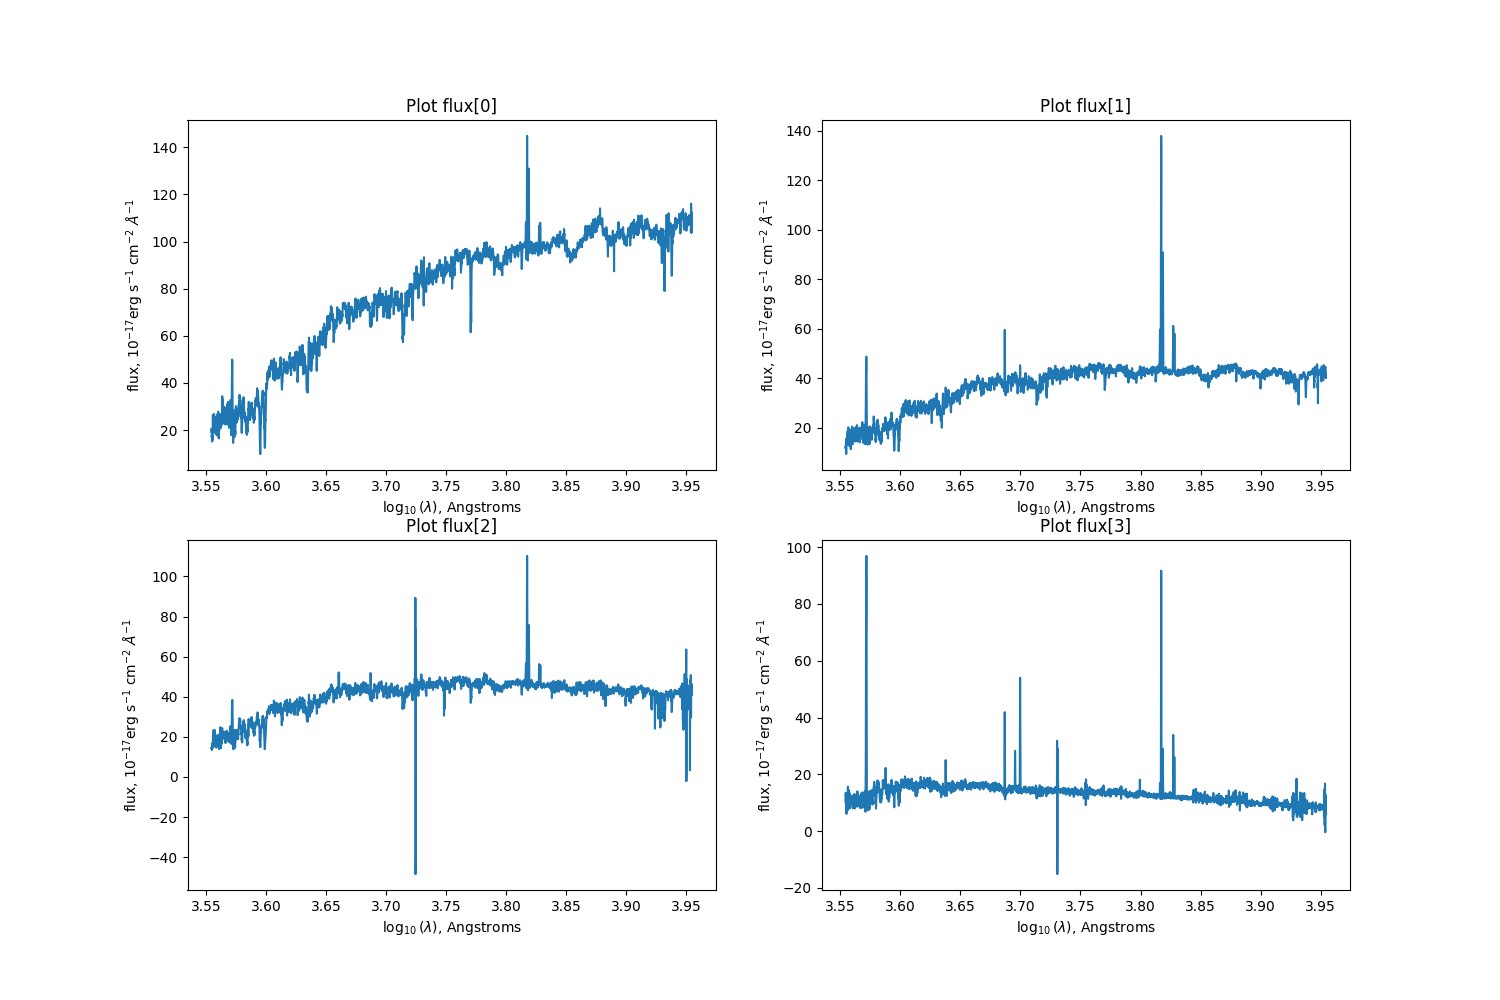
\includegraphics[width=1\textwidth]{Computational Physics/ps6Figures/q1a.png}
\caption{The first four galaxies.}
  \label{fig:Q1a}
\end{figure}

\begin{figure}[b!]
\centering
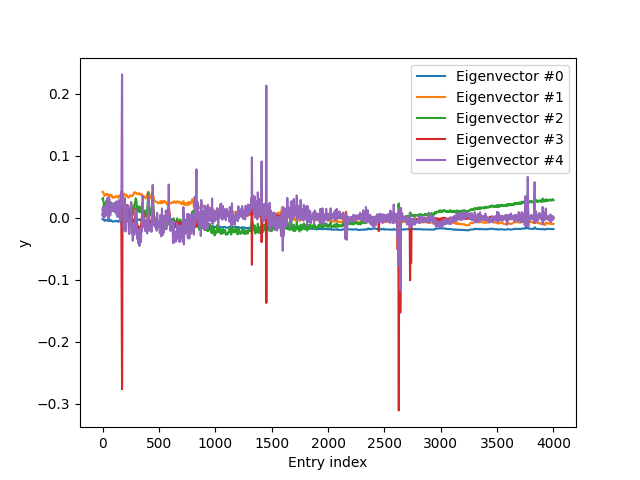
\includegraphics[width=0.6\textwidth]{Computational Physics/ps6Figures/q1d.png}
\caption{The first five eigenvectors of the covariance matrix.}
  \label{fig:Q1d}
\end{figure}

\begin{figure}[b!]
\centering
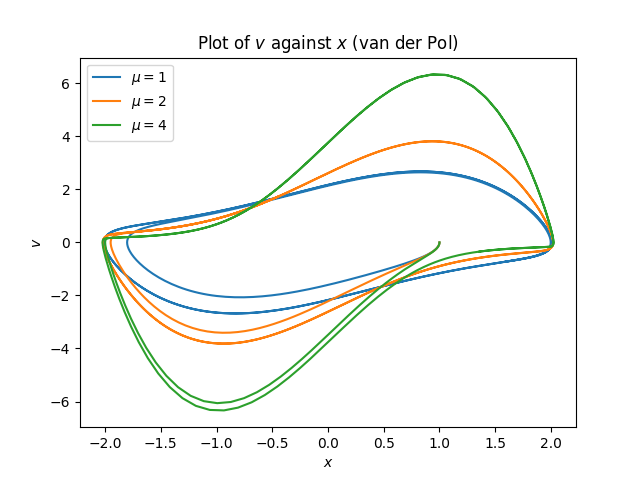
\includegraphics[width=0.6\textwidth]{Computational Physics/ps6Figures/q1e.png}
\caption{Computation time (in seconds) of the covariance matrix method and the SVD method.}
  \label{fig:Q1e}
\end{figure}

\begin{figure}[b!]
\centering
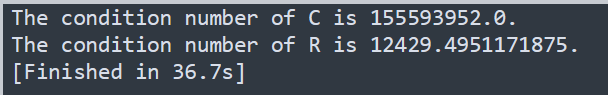
\includegraphics[width=0.6\textwidth]{Computational Physics/ps6Figures/q1f.PNG}
\caption{Condition numbers of $C$ and $R$.}
  \label{fig:Q1f}
\end{figure}

\begin{figure}[b!]
\centering
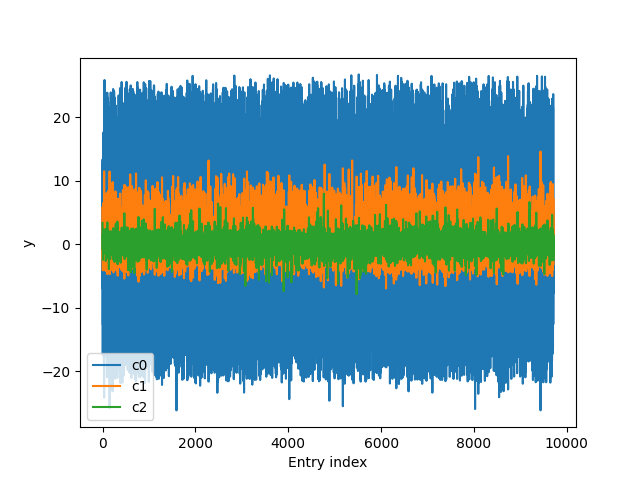
\includegraphics[width=0.6\textwidth]{Computational Physics/ps6Figures/q1h.png}
\caption{$c_0$, $c_1$, and $c_2$ of the PCA.}
  \label{fig:Q1h}
\end{figure}

\begin{figure}[b!]
\centering
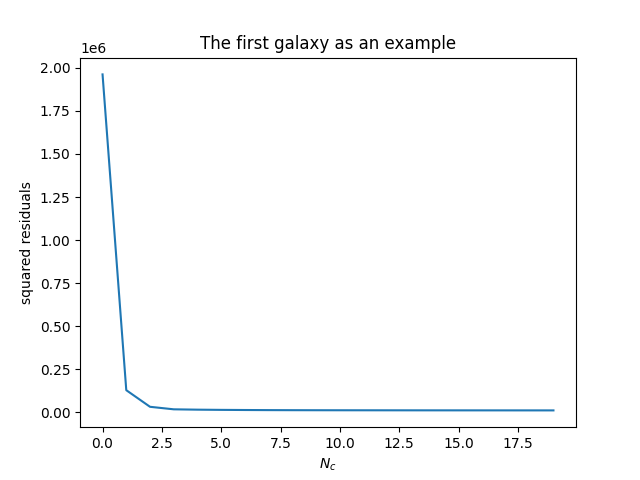
\includegraphics[width=0.6\textwidth]{Computational Physics/ps6Figures/q1i.png}
\caption{The squared residuals between the spectra and the reconsituted, approximate spectra as a function of $N_c$.}
  \label{fig:Q1i}
\end{figure}

\begin{figure}[b!]
\centering
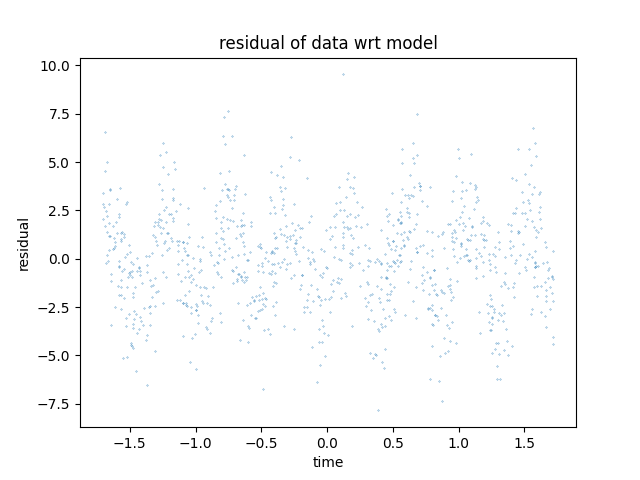
\includegraphics[width=0.6\textwidth]{Computational Physics/ps5Figures/q3c.PNG}
\caption{Q3(c): The residuals of the data wrt the model in part (b).}
  \label{fig:Q3c}
\end{figure}

\begin{figure}[b!]
\centering
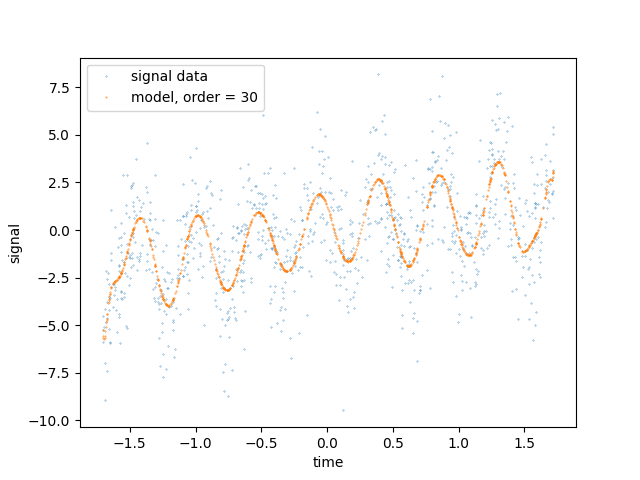
\includegraphics[width=0.6\textwidth]{Computational Physics/ps5Figures/q3dFit.png}
\caption{Q3(d): The signal data and the model with the order of polynomial = 30.}
  \label{fig:Q3dFit}
\end{figure}

\begin{figure}[b!]
\centering
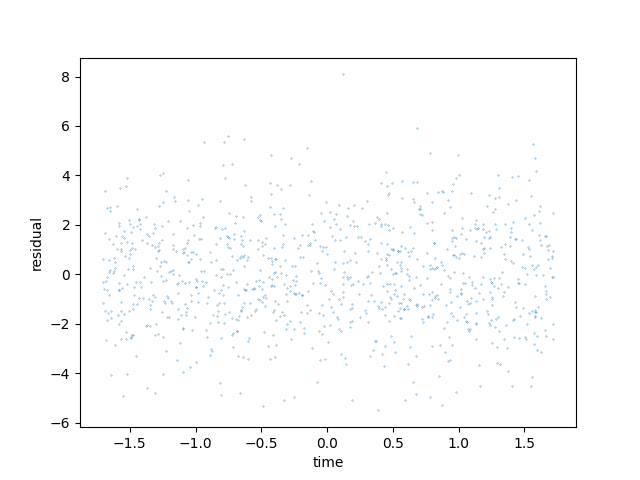
\includegraphics[width=0.6\textwidth]{Computational Physics/ps5Figures/q3dResidual.png}
\caption{Q3(d): The residuals of the data wrt the model with the order of polynomial = 30.}
  \label{fig:Q3dResidual}
\end{figure}

\begin{figure}[b!]
\centering
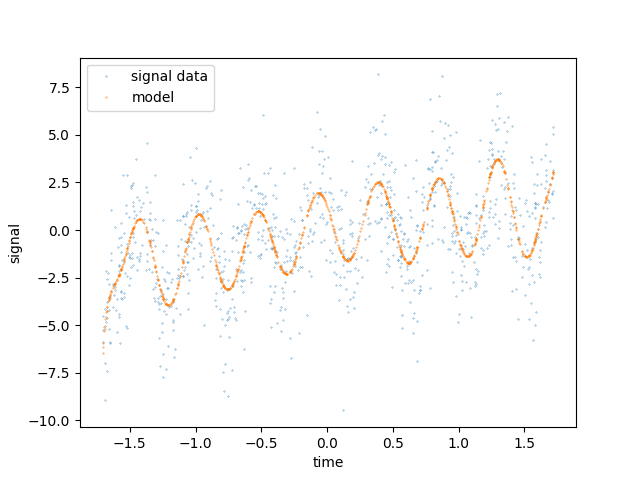
\includegraphics[width=0.6\textwidth]{Computational Physics/ps5Figures/q3eFit.png}
\caption{Q3(e): Use the Lomb-Scargle model to fit the data.}
  \label{fig:Q3eFit}
\end{figure}

\begin{figure}[b!]
\centering
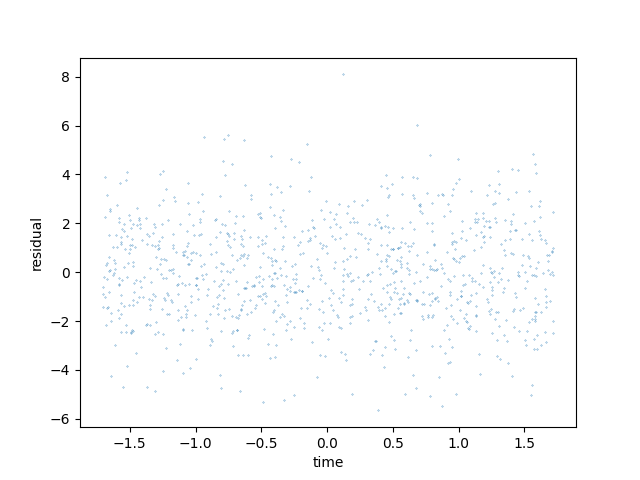
\includegraphics[width=0.6\textwidth]{Computational Physics/ps5Figures/q3eResidual.png}
\caption{Q3(e): The residuals of the data wrt the Lomb-Scargle model.}
  \label{fig:Q3eResidual}
\end{figure}

\bibliographystyle{apj}
\bibliography{example}

\end{document}

 
 
